\begin{frame}[fragile]
  \frametitle{遇到的问题}
  \framesubtitle{背景介绍}

  在“用户画像”数据的读取中,使用了一个由同事开发的工具,通过接口来读取由由定位团队挖掘出来的用户 “家和公司” 的位置。 
  \vspace{\baselineskip}

  由于接口使用了  pbrpc 协议,所以无法通过简单地方式访问,所以我们使用了导航团队同事开发的一个工具(bin,无源码)来读取数据,然后通过脚本去处理该工具输出的方式来协作。 
  \vspace{\baselineskip}

  \pause
  在脚本运行之后,我们拿到了这样一些结果

\end{frame}

\begin{frame}[fragile]
  \frametitle{日志格式}
  \framesubtitle{背景介绍}
  \begin{verbatim}
    cuid:("武汉市","厦门市","重庆市","上海市","广州市","深圳市","成都市","杭州市")
    cuid:00000000000000000000000000000000
    1 10000000.000000 3000000.000000
    0 10000000.000000 3000000.000000
    cuid:00000000000000000000000000000001
    cuid:00000000000000000000000000000002
    cuid:00000000000000000000000000000003
    1 10000000.000000 3000000.000000
  \end{verbatim}
\end{frame}

\begin{frame}[fragile]
  \frametitle{日志格式}
  \framesubtitle{背景介绍}
  由于对应的工具,并没有详细的文档介绍,我们只能通过同事介绍,这份日志的格式做如下描述:

  
  \begin{itemize}
  \item 日志的第一行,是一些 debug 信息
  \item 日志第二行开始,是一系列的 cuid 的查询结果
  \item[-] 以 cuid 开始的行,表示一个结果的开始
  \item[-] 以``1'' 开始的行,表示用户``家'' 的查询结果
  \item[-] 以``0'' 开始的行,表示用户``公司'' 的查询结果
  \item[-] 未附有查询结果的 cuid, 表示未找到对应的值
  \end{itemize}
\end{frame}

\begin{frame}[fragile]
  \frametitle{状态机}
  \framesubtitle{背景介绍}
  对于这样一份看起来很规则很简洁的日志,我们看看它的状态机是什么样的: \pause
  \begin{figure}[htbp]
    \centering
    \includegraphics[scale=.4]{imgs/log_state_trans.png}
    \caption{日志状态机}
    \label{fig:loc-trans}
  \end{figure}
\end{frame}

\begin{frame}[fragile]
  \frametitle{日志处理}
  \framesubtitle{背景介绍}
  可以看出,即使是很简单的日志文件,它的状态机画出来,也会有很多的边界 case 需要关注。
  \begin{figure}[htbp]
    \centering
    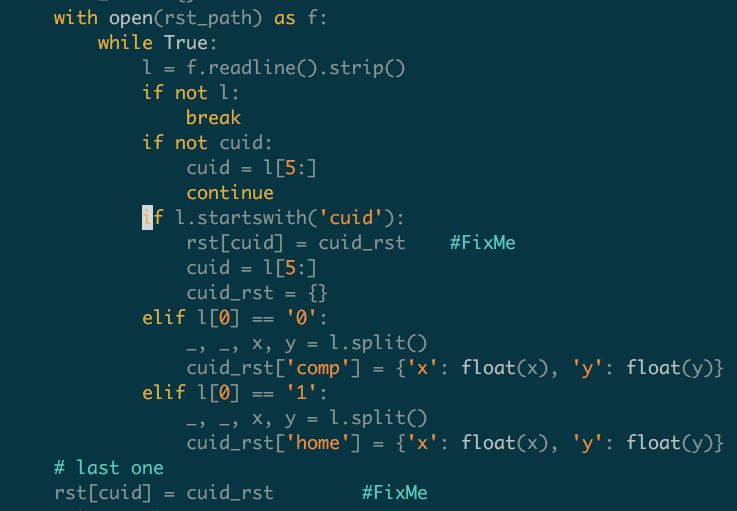
\includegraphics[scale=.3]{imgs/py-regular.png}
  \end{figure}
\end{frame}

\begin{frame}[fragile]
  \frametitle{Cons}
  \framesubtitle{背景介绍}
  根据状态机直接编写处理程序,会遇到以下问题:
  
  \begin{itemize}
  \item 在规则比较复杂的时候,对应的程序有太多分支要处理
  \item 规则很小的变化,可能导致程序变动很大
  \item 很多“可选项”(比如用户家和公司的地址可能不存在)会让程序变得很长
  \item 混合了文本处理与“规则”本身的处理,没有相应介绍不太容易维护
  \end{itemize}
\end{frame}

\begin{frame}[fragile]
  \frametitle{一个 parser 介绍}
  \framesubtitle{Parser}
  下面是另一种“文本”的处理方式,\\ mysql 描述 ``alter database'' 的方式:
  
  \begin{verbatim}
    ALTER {DATABASE | SCHEMA} [db_name]
    alter_specification ...
    ALTER {DATABASE | SCHEMA} db_name
    UPGRADE DATA DIRECTORY NAME

    alter_specification:
    [DEFAULT] CHARACTER SET [=] charset_name
      | [DEFAULT] COLLATE [=] collation_name
  \end{verbatim}
\end{frame}

\begin{frame}[fragile]
  \frametitle{BNF}
  \framesubtitle{Parser}

  Mysql 的文档中,使用了 “BNF” 来描述 sql 的语法,可以把很复杂的、难以表述清楚的规则,完整、清晰的描述,同时保持了简洁。

  \vspace{\baselineskip}

  下面我们尝试使用同样的方式来描述一下前面我们处理的日志
  
\end{frame}

\begin{frame}[fragile]
  \frametitle{BNF}
  \framesubtitle{Parser}
  \begin{verbatim}
    debug_info cuid_rsts

    debug_info:
    cuid:rest_of_line

    cuids_rsts:
    cuid_rst | cuid_rst cuid_rsts
    
    cuid_rst:
    cuid: cuid_value [home_rst [company_rst]]
    
    home_rst:
    1 x_value y_value
    company_rst
    0 x_value y_value
  \end{verbatim}
\end{frame}

\begin{frame}[fragile]
  \frametitle{日志处理}
  \framesubtitle{Parser}
  市面上有很多 parser 相关的工具、库,我们随便选择一种,看看使用一个 parser 怎样处理前面的程序日志,并比较一下跟普通的写的处理程序相比的优缺点。   \\
  \pause
  \vspace{\baselineskip}
  我们选取了 Python 的一个库: pyparsing
  \verb|http://pyparsing.wikispaces.com/|
\end{frame}

\begin{frame}[fragile]
  \frametitle{日志处理}
  \framesubtitle{Parser}
  那这样一份日志:
  \begin{figure}[htbp]
    \centering
    \includegraphics[scale=.4]{imgs/log_state_trans.png}
    \caption{日志状态机}
    \label{fig:loc-trans}
  \end{figure}
\end{frame}

\begin{frame}[fragile]
  \frametitle{日志处理}
  \framesubtitle{Parser}
  在 Python 下是这样描述的:
  %% \begin{lstlisting}[language=Python]
  \begin{verbatim}
    ld, hld, cld = 'cuid:', '1', '0'

    loc_coor = Regex(r'\d+(\.\d*)?([eE]\d+)?')
    loc_rst = loc_coor + loc_coor
    home_rst = Group(hld + loc_rst)('expression')
    comp_rst = Group(cld + loc_rst)('expression')
    rst = Group(ld + Regex(r'[^ ]*') + Optional(home_rst) + \
          Optional(comp_rst))('expression')
    
    rsts = OneOrMore(rst)
    ldline = Group(restOfLine)('expression')
    rst_str = ldline + rsts
  \end{verbatim}
  
\end{frame}


\begin{frame}[fragile]
  \frametitle{日志处理}
  \framesubtitle{Parser}
  描述完成后,可以按照下面的方式来使用:

  \begin{verbatim}
    with open('src.txt') as  f:
    c = f.read()
    rst = rst_str.parseString(c)
    for i in  rst:
       print i
  \end{verbatim}
\end{frame}

\begin{frame}[fragile]
  \frametitle{日志处理}
  \framesubtitle{Parser}
  它生成的结果,是这样的:

  \begin{verbatim}
    with open('src.txt') as  f:
    c = f.read()
    rst = rst_str.parseString(c)
    for i in  rst:
       print i
  \end{verbatim}
\end{frame}


\begin{frame}[fragile]
  \frametitle{Pros and Cons}
  \framesubtitle{Parser}
  
  使用一些 parser 工具,可以在下面几个方面提高工作效率:
  
  \begin{itemize}
  \item 将工作的注意力由原始的文本处理,迁移到抽象后的业务中来,摆脱这些繁琐的细节, 这一点在日志格式复杂的时候,显得尤其重要
  \item 日志的格式发生某种变化的时候,可以通过修改日志定义部分的实现完成适配,不会影响程序其他部分
    \item 与手写的日志处理程序相比,代码更清晰,程序也更容易维护
  \end{itemize}

  当然,parser 也会(在某些场景下) 造成如下困扰:
  
  \begin{itemize}
  \item 有一些学习成本
    \item 根据 parser 本身的实现、文本格式的复杂程度,性能跟裸的处理程序相比可能会有一定下降
  \end{itemize}
\end{frame}

\begin{frame}[fragile]
  \frametitle{Pros and Cons}
  \framesubtitle{Parser}
  
  根据我自身的体会,使用这类工具,可以大大节省开发的时间,同时降低维护成本,如果你的程序的瓶颈不是在日志处理这一部分,非常值得在工作中使用 parser。\\
  下面列举一些常用到的工具以及对应的语言:
  
  \begin{itemize}
  \item pyparsing (Python)
  \item Lex (C)
  \item XXLex(XX代表你使用的语言,比如 Jlex)
  \end{itemize}
\end{frame}

